%%!TEX encoding = UTF-8 Unicode

\documentclass[oneside]{ntuthesis}

\usepackage[utf8]{inputenc}

% Use biblatex instead of bibtex
\usepackage[backend=bibtex, style=ieee]{biblatex}
%% Add all bib source files
\addbibresource{bib/articles.bib}
\addbibresource{bib/books.bib}
\addbibresource{bib/electronic.bib}
\addbibresource{bib/inproceedings.bib}
\addbibresource{bib/proceedings.bib}

\usepackage{mystyle}

%% Disable this package after finishing editing
\usepackage[disable]{todonotes}

% Type your personal information
%% Chinese
%\setUniversityZH  {國立臺灣大學} 
\setCollegeZH     {電機資訊學院}
\setInstituteZH   {電機工程學研究所}
\setThesisTypeZH  {碩士論文}
\setTitleZH		  {網頁和手機程式自動化測試智能技術}
\setAuthorZH      {吳啟允}
\setAdvisorNameZH {王~凡}
\setAdvisorTitleZH{博士}
\setGradYearZH    {105} % The date is generated using \today
\setGradMonthZH   {7}   % You can un-comment and specify the date

%% English
\setUniversityEN  {National Taiwan University}
\setCollegeEN     {College of Electrical Engineering and Computer Science}
\setInstituteEN   {Graduate Institute of Electrical Engineering}
\setThesisTypeEN  {Master Thesis}
\setTitleEN		  {Intelligent Techniques for Automated Testing of Web and Mobile Applications}
\setAuthorEN      {Chi-Yun Wu}
\setAdvisorNameEN {Farn Wang}
\setAdvisorTitleEN{Ph.D.}
%\setGradYearEN    {2015} % The date is generated using \today
%\setGradMonthEN   {June} % You can un-comment and specify the date


\begin{document}
\begin{CJK*}{UTF8}{bkai}

\frontmatter
\maketitle   % Generate title page

%在這裡附圖(口試審定書)
% Dummy chapter for generating ToC
%\addcontentsline{toc}{chapter}{口試委員會審定書}
%
\includepdf[pages={1},pagecommand={}]{official/approvalZH-with-sign}
%\addcontentsline{toc}{chapter}{Oral Examination Approval Form}
%
\includepdf[pages={1},pagecommand={}]{official/approvalEN-with-sign}

\begin{onehalfspace}

\chapter{誌謝}

\setlength{\parindent}{2em}
首先最先感謝我的父母,
有了爸爸媽媽的支持與照顧,
在我低潮的時候鼓勵我勉勵我,
我才能順利完成我的學業。
我也要特別感謝指導教授王凡老師,
總是為我指引研究的方向。
老師教導我軟體測試的專業知識,
也教導我進行研究的方法和態度,
還提供許多機會讓我開廣見聞。
我還要感謝俊偉學長、庭芬學姊和汶宏學長,
因為他們的幫助,
我才能順利完成程式的開發,
對於程式的觀念也進步許多。
我也要感謝修博、宗儒和上誼,
這兩年一起修課,
在困難的時候一起扶持,
一起面對挑戰,
因為有你們的幫助,
我才能堅持完成這一切。
最後感謝所有實驗室的同學,
帶給我歡樂的研究室生活。
謝謝大家。








\end{onehalfspace}

\begin{onehalfspace}
\newcommand{\eng}[1]{\ \raisebox{1pt}{#1}}

\chapter{摘要}。

關鍵字:網頁測試、自動測試

\end{onehalfspace}

\begin{doublespace}

\chapter{Abstract}


Key words: software testing, test automation

\end{doublespace}

\begin{doublespace}
\tableofcontents
\listoffigures
\listoftables
\end{doublespace}


\mainmatter
\begin{doublespace}

\chapter{Introduction}\label{ch:introduction}

\section{Motivation}

Web Applications become more and more indispensable in our life.
People can easily get informations with the development of the Internet.
It becomes more convenient for people to search new knowledge, buy goods and chat with friends.
People spent lots of time on the Internet for working, studying, shopping, socialozong and playing.
As the result, more engineers tend to develop the applications on the Internet.
On the other hand, Mobile Applications is also a choice for software developer.
People can carry smart phone and enjoy the applications everywhere.
Although people can visit web applications by browser on the smart phone,
a special mobile application has a better performance.
Companies may develop the applications on both the Internet and the mobiles.
For instance, Google and Facebook.

In order to guarantee the performance and user experience of the applications,
the testing of the applications is required.
However, the current techniques of testing take lots of works and times.
Because the applications are complex and dynamic,
they have different reaction with different inputs.
Engineers need to write the test scripts case by case according to each functions.
they also need basic knowledge of software testing.
To reduce the work time of testing, the automated testing become essential for engineers.
But the challenge is it is too difficult to generate test case on black box testing.
Without the detailed information of functions,
We may not know how to make a test script.

%介紹software testing,其中又有web testing和mobile APP testing
%software變化大,需要測試確保功能正常,但製作testcase耗費時間人力
%auto testing的好處: 節省人力 black-box testing的好處:應用到所有APP
%建立一個auto testing ,開發者可減輕開發成本


\section{Purpose}

In this paper, we propose a technique to automatically generating traces on dynamic web applications.
The program named WebTraceCollector can collect the informations on web page and try to guess the suitable inputs.
We construct a inputs databank with some examples of inputs,
so the program will find a similar example as the input value of web page.
With the suggested input values,
the program can explore the website automatically and build the finite state machine to represent the website,
and generate the traces for testing.


In order to automatically evaluate traces collected from web and mobile applications,
we propose a teachnique to transform the traces into standard format.
We constrcut a label dictionary, which collects common sense of action and screen from applications,
so the traces can be expressed in a standard vector of labels.
Then, we use the method of machine learning to evaluate traces.
We use SVM to classify the traces into passed traces and failed traces.


%本篇建立了一個auto web testing的工具,和測試web,APP並驗證的framework
%framework將testcase取出symbolic label,train出所有APP可通用的model來evaluate all traces 


\section{Organization}

The rest of this paper is organized as follows.
Chapter 2 shows the related work, 
and we introduce the tool for generating mobile traces and the method used for evaluating in Chapter 3.
In Chapter 4, we propose a technique to generate traces on dynamic web applications.
Chapter 5 shows the framework to evaluate traces from the web and mobiles.
Then, the experiment results shown on the Chapte 6,
and the conclusion in Chapter 7.

%第二章 related work: 其他web,APP tesing, ex: selenium,crwaljax,splinter,Jmeter,UIautomata...
%第三章 preliminaries: machine learning,, test evaluation
%第四章
%第五章



\chapter{Related Works}\label{ch:related}

本篇測試的目標是web 和 Android APP,列出常見的testing 工具

\section{Web testing}

selenium,jmeter 需要先建立testcase 再重複測試

VeriWeb,CrawlJax可自動explore website,建立DOM tree,用DOM建state-based testing

\section{Android testing}

Ranorex,UIautomator 可測試Android APP

ADAutomation: behavior testing, GUI testing

\section{test evaluation}

test oracle use on software testing, finite state machine
% Barr [8]
metamorphic relations, 
Daikon


\chapter{Preliminaries}\label{ch:preliminaries}


\section{SpecElicitor}

SpecElicitor is a tool made by Yuan-Hong Lo, 
which can help user test Mobile Application with friendly GUI interface.

When user start using SpecElicitor,
each time user do an action on the Mobile Application, 
the tool will ask for labeling the action and the screen shown on the interface.
The interface is shown in Fig[].
By using SpecElicitor, we can choose the specified action at every step, label the meaning of the action,
and label the exception situation if it happen and stop the trace at any time we need.
The interface of the SpecElicitor is shown in Fig[\ref{SpecElicitorInterface}].


The traces made by SpecElicitor include automata, screenshots, XML files and labels.
The automata is a json file record every states and edges on the traces.
A state has a screenshot and a XML file dumped from the Mobile.
A edge records the action user did such as clicking element, typing text or exiting the Application.
The traces also record labels on every states and edges,
so we can recognize how many label we focus on happened on the trace.
An example trace of Recipe Application made by SpecElicitor is shown in Fig[\ref{SpecElicitorTraces}].

%Our LAb 建立了一個工具SpecElicitor
%使用者可以在GUI介面下一邊建立APP的trace, 同時標記該畫面/動作的label
%使用完後會產生含有 XML, 截圖, label的traces

\begin{figure}[h]
	\graphicspath{{pic/}}
	\begin{center}
		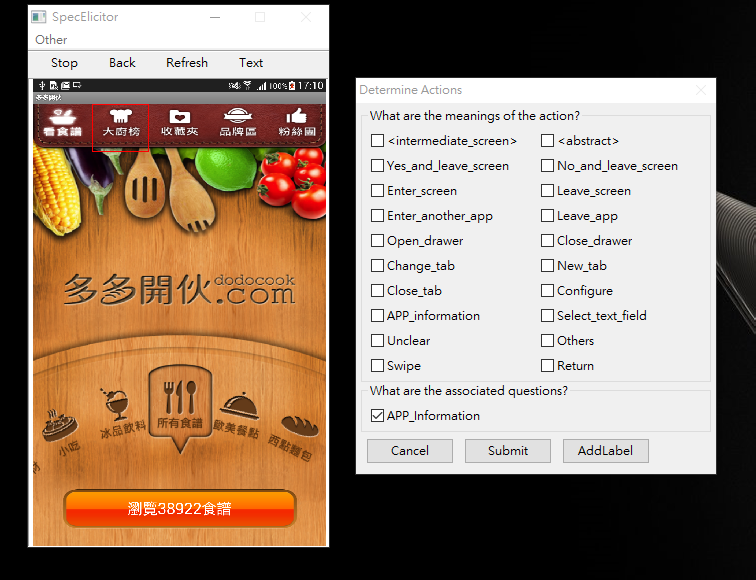
\includegraphics[width=0.8\textwidth]{SpecElicitorInterface.png}
		\caption{ The GUI interface of SpecElicitor.  }
		\label{SpecElicitorInterface}
	\end{center}
\end{figure}

\begin{figure}[h]
	\graphicspath{{pic/}}
	\begin{center}
		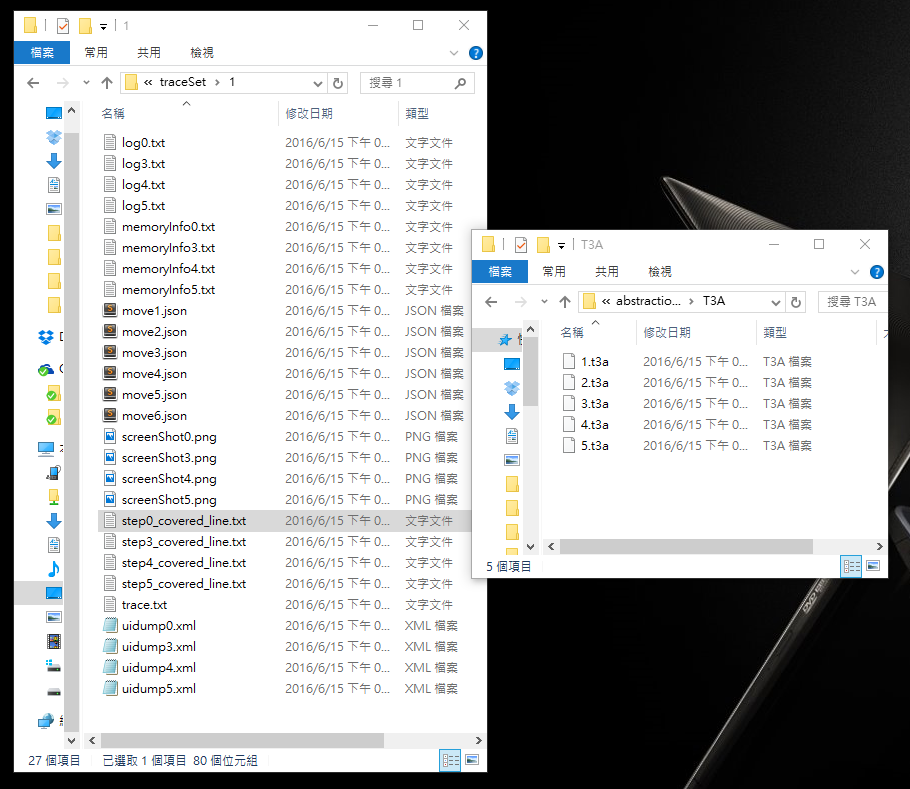
\includegraphics[width=0.8\textwidth]{SpecElicitorTraces.png}
		\caption{ An example of the traces.  }
		\label{SpecElicitorTraces}
	\end{center}
\end{figure}

\clearpage

\section{Common Sense Model}

將APP建立出state-base的automata,其中screen作為state,action作為edge

用統一的normalized terms來specific

our Lab建立一個TAAD的SpecElicitor,可產生label的trace


\section{Support Vector Machine}

SVM 在高維度 用largest margin來 seperate datas 

SVM可用來 cluster data

\chapter{Overview}\label{ch:overview}


%\subincludefrom{tex/}{ch-proving}

\chapter{Experiments}\label{ch:experiments}

We construct a tool WebTraceCollector for automatic web testing,
which can explore the website automaically and 
analyze the DOM tree of the current web page to find the next clickable element to click,
and propose a machine learning method to evaluate traces by SVM.
In order to use the tool and implement the evaluation, wee need a laptop and installing some tools.
The specification of the laptop we used is shown in Table[\ref{laptopSpec}],
and we need to install Windows, Python 3.4.3 and MySQL database.

\begin{table}[ht]
	\begin{center}
		\begin{tabular}{| l | l | }
			\hline
			Laptop & AUSU X450JN \\ \hline
			Operating System & Windows 10 (64bit) \\ \hline
			CPU & Intel(R) Core(TM) i5-4200 @2.8GHz \\ \hline
			RAM & 4GB \\ \hline
			Storage & 800G \\ \hline
		\end{tabular}
		\caption{ The specification of the laptop. }
		\label{laptopSpec}
	\end{center}
\end{table}

WebTraceCollector is constructed based on Python,
it control the browser by the selenium library and recognize the elements of the current page by the beautifulsoup library.
The automatic exploring mechanism highly depends on the page source downloaded from the current web page.
If the page source ot the constructed DOM tree can not match the current page correctly,
we can not find the correct clickable element and the testing may fail.
Thus, it is important to check how many web applications can download page soucre and construct DOM tree accurately.
In the experiment 1, we find 20 websites which is famous in taiwan.
We test those websites and generate traces automatically by WebTraceCollector.
Moreover, we want to check the ability of handling dynamic web pages.
We choose some common web pages with lots of input fields need to be inserted to test in the experiment 2.
In the experiment 3, we want to check the accuracy of the automatic prediction.
We generate some traces of certain applications and use those traces to train SVM model,
and we use this model to predict the traces of the applications.

\section{Trace collection}

In 20 popular applications\cite{popularWebs} that shown in Table \ref{popularWebs},
there are forums, news, community platforms, games and blogs.
We generate monkey traces by randomly click buttons and the length of traces is about 5.
The reason that we do not completely explore the whole website is most of the scale of websites are too big.
For example, a news website may have thousands of subpages and it may cost too much time to generate completely traces.
We just want to check the DOM tree is constructed correctly, 
so we make short traces to focus on checking the ability of clicking correct clickable elements.

The result of the experiments is shown in Table[].
There are 4 web applications that have serious problem on testing,
and most of web applications can be successfully explored with little defects.
There are two unkown fail happened, however it can work after restart the test.
The problems of the fail applications are 
too many iframes of advertising and API plugin in the webpages and buttons functions implemented by javascript.
The iframes become noise in the page source and make the DOM tree constructed incorrectly,
so WebTraceCollector may not find the correct clickable elements or only focus on the clickables in the advertising iframe.
On the other hand, the button functions in the web pages may implemented by javascript.
That means clickable elements may not be the style we thought, such as link tags or input-button tags,
it could be images, div tags or any tags if javascript bind the mouse listener on.
With the uncertain clickable elements, it is hard to find the correct clickable elements to explore the web and record the traces.
WebTraceCollector will click the wrong elements with nothing happens and stay at the same page until the trace is end.

\begin{table}[ht]
	\begin{center}
		\begin{tabular}{ | l | l | l | l | }
			\hline
			編號 & 網站名稱 & 網站類型 & URL \\ \hline
			1 & Facebook & Community platform & https://www.facebook.com/ \\ \hline
			2 & YouTube & Entertainment & https://www.youtube.com/ \\ \hline
			3 & Yahoo & Search engine & https://tw.yahoo.com/ \\ \hline
			4 & Google & Search engine & https://www.google.com.tw/ \\ \hline
			5 & 中時電子報 & News & http://www.chinatimes.com/ \\ \hline
			6 & 露天拍賣 & Commerce & http://www.ruten.com.tw/ \\ \hline
			7 & 聯合新聞網 & News & http://udn.com/news/index \\ \hline
			8 & 巴哈姆特 & Forum & http://www.gamer.com.tw/ \\ \hline
			9 & Mobile01 & Forum & http://www.mobile01.com/ \\ \hline
			10 & 蘋果日報 & News & http://www.appledaily.com.tw/ \\ \hline
			11 & 百度 & Search engine & https://www.baidu.com/ \\ \hline
			12 & 東森新聞雲 & News & http://www.ettoday.net/ \\ \hline
			13 & 卡提諾論壇 & Forum & http://ck101.com/ \\ \hline
			14 & 伊莉討論區 & Forum & http://www40.eyny.com/index.php \\ \hline
			15 & Hinet & Search engine & http://www.hinet.net/ \\ \hline
			16 & 微軟Live.com & Search engine & https://login.live.com/ \\ \hline
			17 & 痞客邦 & Blog & https://www.pixnet.net/ \\ \hline
			18 & PChome Online & Search engine & http://pchome.com.tw/ \\ \hline
			19 & 淘寶 & Commerce & https://world.taobao.com/ \\ \hline
			20 & Life生活網 & Blog & http://www.life.com.tw/ \\ \hline
			21 & 104人力銀行 & Survice & http://104.com.tw/ \\ \hline
			22 & 騰訊網  & Search Engine & http://www.qq.com/ \\ \hline
			23 & 新浪微博 & Community platform & http://www.weibo.com/login.php \\ \hline
			24 & 自由時報電子報 & News & http://www.ltn.com.tw/ \\ \hline
			25 & 維基百科 & Dictionary & https://www.wikipedia.org/ \\ \hline
		\end{tabular}
		\caption{ The 20 popular websites. }
		\label{popularWebs}
	\end{center}
\end{table}

\begin{table}[ht]
	\begin{center}
		\begin{tabular}{ | l | l | l | l | }
			\hline
			26 & 博客來 & Commerce & http://www.books.com.tw/ \\ \hline
			27 & 今日新聞網 & News & http://www.nownews.com/ \\ \hline
			28 & 商業周刊 & News & http://www.businessweekly.com.tw/ \\ \hline
			29 & 隨意窩Xuite & Blog & http://xuite.net/ \\ \hline
			30 & 1111人力銀行 & Survice & http://www.1111.com.tw/ \\ \hline
			31 & Flickr & Community platform & https://www.flickr.com/ \\ \hline
			32 & Blogger & Blog & http://www.blogger.com/ \\ \hline
			33 & 批踢踢實業坊 & Community platform & https://www.ptt.cc/index.html \\ \hline
			34 & FC2 & Survice & http://fc2.com/ \\ \hline
			35 & 卡卡洛普 & Survice & http://www.gamme.com.tw/ \\ \hline
			36 & PChome商店街 & Commerce & http://www.pcstore.com.tw/ \\ \hline
			37 & Giga Circle & Survice & http://tw.gigacircle.com/ \\ \hline
			38 & 鉅亨網 & News & http://www.cnyes.com/ \\ \hline
			39 & momo購物網 & Commerce & http://www.momoshop.com.tw/main/Main.jsp \\ \hline
			40 & 蕃薯藤 & Search engine & http://www.yam.com/ \\ \hline
			41 & OB嚴選 & Commerce & http://www.obdesign.com.tw/ \\ \hline
			42 & GOMAJI & Commerce & http://www.gomaji.com/Taipei \\ \hline
			43 & 愛評網 & Survice & http://www.ipeen.com.tw/ \\ \hline
			44 & 123KUBO酷播 & Entertainment & http://www.123kubo.com/ \\ \hline
			45 & 591租屋網 & Commerce & https://www.591.com.tw/ \\ \hline
			46 & TEEPR趣味新聞 & News & http://www.teepr.com/ \\ \hline
			47 & KKBOX & Entertainment & https://www.kkbox.com/tw/tc/index.html \\ \hline
			48 & msn台灣 & Search Engine & http://www.msn.com/zh-tw/ \\ \hline
			49 & 微軟 & Survice & https://www.microsoft.com/zh-tw/ \\ \hline
			50 & T客邦 & Blog & http://www.techbang.com/ \\ \hline
		\end{tabular}
	\end{center}
\end{table}

%針對20個網站做20個monkey traces的結果
%有些網站太複雜 iframe太多,太相似

\clearpage

\section{Dynamic webpages}

In order to test the ability of explore dynamic webpages,
we select some webpages that have lots of input fields and it need to insert correct values to pass through the web pages.
The selected webpages are shown in Table \ref{DynamicWebs}.
Most of the input fields in those web pages are names, years, emails and so on.
We can see that there are 4 web pages can be successfully passed through, but 3 web pages can not.
There are 3 reasons that can not pass through the dynamic web pages are the follows:
\\	1. The web pages have robot checking mechanism to prevent automatic exploring.
\\	2. The form of input fields are different to the examples in the database.
\\	3. The input fields are out of the range of examples we collecteed.
	
In reason 1, the robot checking like image recognition is developed to prevent people exploring the website automatically be computer.
It is too hard to find out the correct value by program,
and it is unreasonable if we can easily pass through those web pages.
If we want to test those websites,
the reasonable way is let the developers of the websites turn off the robot ckecking.

In reason 2, even though we have collect the examples of the input fields in the database, 
it is still a hard work to find out the correct form of the values.
For instance, we analyze the input field and find out the value should be a string of address.
But the type of input fields can be text, checkbox or selects, 
it is too hard to analyze user should insert the whole string of address or select each partens of area.

In reason 3, the web pages can have unlimited kinds of input fields.
Although we can add as more examples and rules in the database as we possible,
it is still impossible to handle all kinds of input fields by only few kinds of examples.
In future work, we can develop to find out the values by other method such as maching learning.

\begin{table}[ht]
	\begin{center}
		\begin{tabular}{ | l | l | }
			\hline
			URL & Result \\ \hline
			http://www.plurk.com/signup & Pass \\  \hline
			https://ups.moe.edu.tw/Personal\_Page/index.php & Pass \\  \hline
			https://applyweb.collegenet.com/account/new/create  & Pass \\  \hline
			https://apply.grad.ucsd.edu/signup  & Pass \\  \hline
			https://user.gamer.com.tw/regS1.phpt  & Fail \\  \hline
			http://panel.pixnet.cc/signup/step2  & Fail \\  \hline   
			https://apps.grad.uw.edu/applForAdmiss/newUserProfile.aspx?bhcp=1 & Fail \\  \hline 
		\end{tabular}
		\caption{ The dynamic webpages. }
		\label{DynamicWebs}
	\end{center}
\end{table}

%針對5個有inputs的網站做traces
%有的網站可以通過 有的只能一次(註冊) 有的偶爾可以(登入) 有的不行

\clearpage

\section{Prediction}

In this experiment, we focus on the ability of automated predicting passed traces and failed traces.
We select two web applications to use in our study and analysis their results.
The first web application is a small website about restraurant with simple buttons, 
and the second web application is a more complex website about APP store.
Before comparing the results of predicting traces between different applications,
we should collect the passed traces and failed traces from those web applications first.
Thus, we generate the random traces automatically by the tool WebTraceCollector introduced above
and select certain buttons and screens as the failed traits.

The traces with the specific buttons or screens will be labeled as failed traces and the other traces will be labeled as passed traces.
The detailed information of traces collected from the two web applications is shown in Table \ref{WebtracesProporiton} .
We can see that the percentage of failed traces is low.
The reason is that if the bugs are not occur at the main functionf of the applications,
there will be only a few traces triggering the bugs.

After collecting traces, the traces should be divided into training set for training SVM model and testing set.
We randomly devide the traces into two sets,
and repeat the experiments with different proportion of training set.
The result of prediction traces of application 1 is shown in Table \ref{PredictResult}.
Notice that the accuracy of prediction may not be better than just predicting every traces to pass,
because the number of failed trace is smaller than the number of passed trace.

Even though the prediction can not enhance the accuracy,
it still can help people finding failed traces.
The precision is the number of traces predicted failed that actually failed devided by the number of traces predicted as failed, 
which means the accuracy of predicting failed trace.
With the higher precision, it will be more convinced the traces predicted to be failed is actually failed.
If the precision is high enough, it can reduce human effort by predicting the failed traces with the convinced model.

The recall is the number of traces predicted failed that actually failed devided by the number of failed traces,
which means the ability of finding the failed traces in all traces.
With the higher recall, it will be more convinced that the system can find all the failed traces.
If the recall is high enough, it can reduce human effort by finding the failed traces with the convinced model.

We can obeserve that the accuracy of prediction in application 1 is about 0.65 ~ 0.75.
The average of precision is about 0.5 and the average of recall is about 0.45 but larger range.
From the result, we can say that the predictive model can find almost half of the failed traces in testing set,
and the half of the predicted traces are actually failed.

The result of prediction traces of application 2 is shown in Table \ref{PredictResult2}.
We can obeserve that the accuracy of prediction in application 1 is about 0.75 ~ 0.85.
The average of precision is about 0.5 and the average of recall is about 0.45 but larger range.
However, there are models that have very low precision and recall in some iterations.
It seems that sometimes SVM can not build a reliable model from training.
Because the web application 2 is more complex than application 1 
and the feature keywords is not precise enough to present the difference between passed traces and failed traces.
It will be hard to learn the predictive model of application 2.
The proportion of negative labels is another problem.
Because the amount of failed traces of application 2 is less than the failed traces of application 1,
The method of deviding traces into training set and testing set has a greater influence on learning model.
If we can not find the most important trace for training,
it will be difficult to learn the model and result in poor outcome.

Although the results of automated prediction shown in the above experiments is not good enough to replace all human effort,
it is still a feasible method for reducing the cost of web application testing.
In order to increase the accuracy of automated predicting,
the future work we need to do is to collect more keywords precisely and find other method of deviding traces into training set.
We can select the traces to trainging set depending on which trace can maximize the feature coverage or which trace has the least confident.
We can also use other machine learning algorithm, such as deep learning, to construct the predictice model.

\begin{table}[ht]
	\begin{center}
		\begin{tabular}{ | l | c | c | c | c | }%對同種類的網站 APP 和WEB 做traces
			\hline%測出其中有BUG
			Web Application & Total traces & Pass traces & Fail traces &  Negative Proportion \\ \hline
			Restraurant & 122 & 86 & 36 & 29.5\% \\ \hline
			APP Store & 94 & 84 & 10 & 10.63\% \\ \hline
		\end{tabular}
		\caption{ The number of passed traces and failed traces. }
		\label{WebtracesProporiton}
	\end{center}
\end{table}


\begin{table}[ht]
	\begin{center}
		\begin{tabular}{ | l | c | c | c | c | }
			\hline
			Application 1 & Training & Accuracy & Precision & Recall \\ \hline
			Repeat 1 & 0.4 & 0.7436 & 0.5  & 0.4  \\ \hline
			Repeat 2 & 0.4 & 0.75   & 0.64 & 0.5  \\ \hline
			Repeat 3 & 0.4 & 0.6486 & 0.5  & 0.46 \\ \hline
			Repeat 4 & 0.4 & 0.7333 & 0.53 & 0.69 \\ \hline
			Repeat 5 & 0.4 & 0.7209 & 0.63 & 0.46 \\ \hline
			Repeat 6 & 0.4 & 0.6667 & 0.45 & 0.45 \\ \hline
			Repeat 7 & 0.4 & 0.6154 & 0.35 & 0.6  \\ \hline
			Repeat 8 & 0.6 & 0.7272 & 0.5  & 0.5  \\ \hline
			Repeat 9 & 0.6 & 0.7307 & 0.5  & 0.43 \\ \hline
			Repeat 10& 0.6 & 0.6667 & 0.6  & 0.43 \\ \hline
			Repeat 11& 0.6 & 0.6087 & 0.43 & 0.38 \\ \hline
			Repeat 12& 0.6 & 0.7407 & 0.67 & 0.45 \\ \hline
			Repeat 13& 0.6 & 0.750  & 0.57 & 0.67 \\ \hline
			Repeat 14& 0.6 & 0.70   & 0.67 & 0.5  \\ \hline
		\end{tabular}
		\caption{ The prediction of Application 1. }
		\label{PredictResult}
	\end{center}
\end{table}

\begin{table}[ht]
	\begin{center}
		\begin{tabular}{ | l | c | c | c | c | }
			\hline
			Application 1 & Training & Accuracy & Precision & Recall \\ \hline
			Repeat 1 & 0.4 & 0.833  & 0.4  & 0.66  \\ \hline
			Repeat 2 & 0.4 & 0.891  & 1.0  & 0.33  \\ \hline
			Repeat 3 & 0.4 & 0.857  & 0.5  & 0.33  \\ \hline
			Repeat 4 & 0.4 & 0.920  & 1.0  & 0.33  \\ \hline
			Repeat 5 & 0.4 & 0.8787 & 0.5 & 0.25   \\ \hline
			Repeat 6 & 0.6 & 0.85   & 0.3  & 0.5   \\ \hline
			Repeat 7 & 0.6 & 0.88   & 0.4  & 1.0   \\ \hline
			Repeat 8 & 0.6 & 0.666  & 0.125& 0.5   \\ \hline
			Repeat 9 & 0.6 & 0.8    & 0.2  & 1.0   \\ \hline
			Repeat 10& 0.6 & 0.6363 & 0.1  & 1.0   \\ \hline
		\end{tabular}
		\caption{ The prediction of Application 2. }
		\label{PredictResult2}
	\end{center}
\end{table}

\chapter{Conclusion}\label{ch:conclusion}
\end{doublespace}

\backmatter
% Bibliography
\begin{doublespace}
\printbibliography
\end{doublespace}

\clearpage\end{CJK*}
\end{document}
